% Ondas electromagneticas

\chapter{Ondas Electromagn\'eticas}
\label{sec:ondas.electromagneticas}

\section{Introducci\'on}
\label{sec:A.00.introduccion}

Este Ap\'endice se ha agregado al texto a fin de 
establecer el escenario y proporcionar una introducción a los principios de los sistemas de comunicación por radio. 
En los diversos cap\'itulos del material de estudio se desarrollan m\'as detalladamente sus aplicaciones a diversos sistemas de las aeronaves.



\section{Un poco de historia...}
\label{sec:A.01.un.poco.de.historia}

La ciencia que se ocupa de estudiar el comportamiento de las ondas de radio se conoce como electromagnetismo. En 1864 el escoc\'es James Clark Maxwell presenta la teoría unificada de la electricidad y el magnetismo fundando la ciencia del Electromagnetismo, fue este trabajo el que preparó el escenario para todos los grandes logros en física, telecomunicaciones e ingeniería eléctrica que iban a seguir. En ella postula que la luz está compuesta por ondas electromagnéticas, pero que pueden existir ondas electromagnéticas en frecuencias distintas a las de la luz. 


15 años después el científico alemán Rudolf Hertz comprueba la teoría planteada por Maxwell y publica su trabajo sobre ondas eléctricas en 1893, logrando fabricar el primer transmisor y receptor que se conoce.

Hertz utilizó una disposición de resonadores rudimentarios para demostrar la existencia de las mismas. Su equipoz era extremadamente simple y comprendía dos bucles resonantes, uno para transmitir y el otro para recibir. Cada bucle actuaba como un circuito sintonizado y como una antena resonante (o ``\emph{aérea}'').

El circuito de transmisión de Hertz se excitó mediante una bobina de inducción y una batería. Parte de la energía irradiada por el bucle de transmisión fue interceptada por el bucle receptor y la energía recibida fue transportada a un espacio de chispa donde podría liberarse como un arco. La energía radiada por el circuito de transmisión tenía la forma de una onda electromagnética, una onda que tiene componentes de campo eléctrico y magnético y que viaja a la velocidad de la luz en el vac\'io.


Estos experimentos fueron conocidos por el empresario y científico Italiano Guillermo Marconi quien desarrolla antenas, transmisores y receptores básicos para lograr transmitir información a través del aire utilizando el código Morse, finalmente encuentra apoyo en el gobierno inglés para construir la primera estación de radio a gran escala y con ello logra comunicación a través del canal de la mancha y posteriormente, en los albores del siglo XIX, logra la primer comunicación transoceánica entre la estación de Poldhu y la estación de San Jhones en Newfoundland en Canadá, en el año 1901.

A partir de ese momento la humanidad entró en una nueva era, ya que la comunicación entre continentes se volvió inmediata y el transporte marítimo entre América y Europa, cuyos barcos se mantenían incomunicados varios meses en los que no se sabía de su destino, finalmente, podían comunicarse con las estaciones costeras utilizando radiocomunicaciones.

El sistema de telegrafía inalámbrica de Marconi demostró ser invaluable para las comunicaciones mar\'itimas (barco a barco y barco a tierra) y result\'o fundamental para salvar muchas vidas. Las aplicaciones militares de la radio se explotaron por primera vez, lamentablemente, durante la Primera Guerra Mundial (1914 a 1918) y, durante ese período, la radio se utilizó, tambi\'en por primera vez, en aeronaves.

\begin{figure}[!htb]
  \centering
  \subfigure[La estación de Poldhu en Cornwall Inglaterra, torres de madera de 70 metros de altura y un transmisor con potencia de 25000 vatios.]{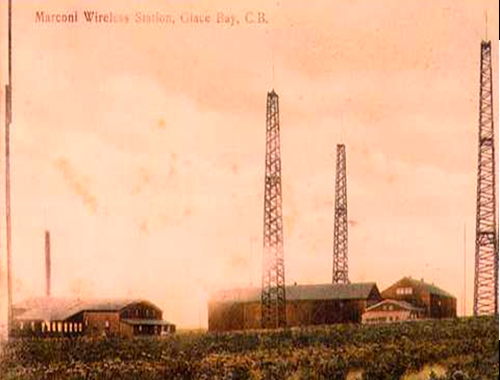
\includegraphics[width=0.40\textwidth]{Apendices/Apendice.A.imagenes/U09_estacion_cornwall_original.jpg}} \hspace{3mm}
\subfigure[Monumento en Saint Jhones, Newfoundland Canada, donde se recibió la primer comunicación interoceánica desde la estación de Pholdu.]{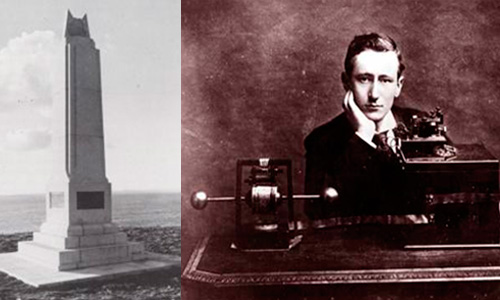
\includegraphics[width=0.50\textwidth]{Apendices/Apendice.A.imagenes/U09_Monumento-en-Saint-Jhones-Newfoundland-Canada.jpg}}

  \caption{Im\'agenes hist\'oricas de radiocomunicaci\'on. %Fuente \cite{historia_radiofrecuencias}
}
  \label{fig:A.imagenes.historicas.radiocomunicacion}
\end{figure}





\section{El espectro de radiofrecuencia}
\label{sec:A.02.espectro.radiofrecuencias}

En general, se entiende que las señales de radiofrecuencia ocupan un rango de frecuencia que se extiende desde unas pocas decenas de kilohercios (kHz) hasta varios cientos de gigahercios (GHz). La parte más baja del rango de radiofrecuencia de uso práctico (por debajo de 30 kHz) solo es adecuada para la comunicación de banda estrecha. A esta frecuencia, las señales se propagan como ondas de tierra (siguiendo la curvatura de la tierra) a distancias muy largas.

En el otro extremo, el rango de frecuencia más alto que es de importancia práctica se extiende por encima de 30 GHz.

En estas frecuencias de microondas existen disponibles anchos de banda considerables (suficientes para transmitir muchos canales de televisión utilizando enlaces punto a punto o para permitir sistemas de radar de muy alta definición) y las señales tienden a propagarse estrictamente a lo largo de las líneas de visión.

En otras frecuencias, las señales pueden propagarse por diversos medios, incluida la reflexión de las capas ionizadas en la ionosfera. A frecuencias entre 3 MHz y 30 MHz, la propagación ionosférica permite regularmente la transmisión y las comunicaciones intercontinentales.

Por conveniencia, el espectro de radiofrecuencia se divide en varias bandas, seg\'un puede observarse en la 
Figura \ref{fig:A.espectro.electromagnetico}
cada una de las cuales abarca una década de frecuencia. El uso que se le da a cada rango de frecuencia depende de varios factores, entre los cuales se encuentran las características de propagación dentro de la banda en cuestión.

Otros factores que deben tenerse en cuenta incluyen la eficiencia de los sistemas aéreos prácticos en el rango en cuestión y el ancho de banda disponible. También vale la pena señalar que, aunque en la Figura \ref{fig:A.espectro.electromagnetico} puede parecer que una gran parte del espectro de radiofrecuencia no se usa, la competencia por el espacio de frecuencia es feroz y, en la pr\'actica hay poco espacio libre.
Las asignaciones de frecuencia son, por lo tanto, ratificadas por acuerdos internacionales y los diversos servicios de usuarios protegen cuidadosamente sus propias áreas del espectro.

\begin{figure}[!htb]
  \centering
  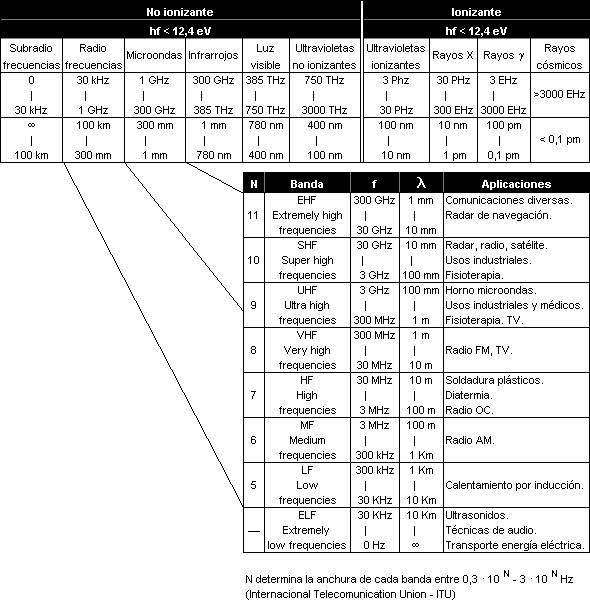
\includegraphics[width=\textwidth]{Apendices/Apendice.A.imagenes/espectro-frecuencias.jpg}
  \caption{Espectro electromagn\'etico}
  \label{fig:A.espectro.electromagnetico}
\end{figure}


\section{Ondas electromagnéticas}
\label{sec:A.03.ondas.electromagneticas}


Al igual que con la luz, las ondas de radio se propagan hacia afuera desde una fuente de energía (transmisor) y comprenden campos eléctricos ($\vec{E}$) y magnéticos ($\vec{H}$) en ángulo recto entre sí. Estos dos componentes, el campo $\vec{E}$ y el campo $\vec{H}$, son inseparables. La onda resultante se aleja de la fuente con las líneas \textbf{E} y \textbf{H} mutuamente en ángulo recto a la dirección de propagación, como se muestra en la Figura 1.2.

Se dice que las ondas de radio están polarizadas en el plano del campo eléctrico ($\vec{E}$). Por lo tanto, si el campo $\vec{E}$ es vertical, se dice que la señal está polarizada verticalmente mientras que, si el campo $\vec{E}$ es horizontal, se dice que la señal está polarizada horizontalmente. La figura 1.3 muestra las líneas eléctricas del campo  $\vec{E}$ en el espacio entre un transmisor y un receptor. La antena del transmisor (un dipolo simple, consulte la página 16) se suministra con una corriente alterna de alta frecuencia. Esto da lugar a un campo eléctrico alterno entre los extremos de la antena y un campo magnético alterno alrededor (y en ángulo recto).

La dirección de las líneas del campo $\vec{E}$ se invierte en cada ciclo de la señal a medida que el frente de onda se mueve hacia afuera desde la fuente. La antena receptora intercepta el campo en movimiento y, como consecuencia, se induce voltaje y corriente en él. Este voltaje y corriente es similar (pero de menor amplitud) al producido por el transmisor. Tenga en cuenta que en la Figura 1.3 (donde el transmisor y el receptor están muy juntos) el campo se muestra desplegado en un patrón esférico (esto se conoce más correctamente como el campo cercano). En la práctica, habrá una distancia considerable entre el transmisor y el receptor, por lo que la onda que llega a la antena receptora tendrá un frente de onda plano. En esta región de campo lejano, la distribución del campo angular es esencialmente independiente de la distancia desde la antena transmisora.


\section{Frecuencia y longitud de onda}
\label{sec:A.04.frecuencia.y.longitud.onda}


Las ondas de radio se propagan en el vac\'io a la velocidad de la luz (300000 kil\'ometros por segundo). La velocidad de propagación, $v$, longitud de onda, $\lambda$ y frecuencia, $f$, de una onda de radio están relacionadas por la siguiente expresi\'on:

\begin{equation}
  \label{eq:A.velocidad.onda}
  v = f\,\lambda = 3\times10^8\,\text{m}/\text{seg}
\end{equation}

Donde $f$ se expresa en Hz = 1/seg y $\lambda$ en metros. 
Esta expresi\'on se puede organizar para que $\lambda$ sea despejada de la siguiente forma:

\begin{equation}
  \label{eq:A.frecuencia.ecuacion}
  f = \displaystyle \frac{3\times10^8\,\text{m}/\text{seg}}{\lambda} \qquad \Longrightarrow \qquad
  \lambda = \displaystyle \frac{3\times10^8\,\text{m}/\text{seg}}{f}
\end{equation}

Como ejemplo, una señal a una frecuencia de 1 kHz ($10^3$ Hz) tendrá una longitud de onda de 300000 m, mientras que una señal a una frecuencia de 1 MHz ($10^6$ Hz) tendrá una longitud de onda de 300 m.

Cuando una onda de radio viaja en un cable (en lugar de en el aire o ``\emph{espacio libre}''), su velocidad generalmente se reduce entre un 60\% y 80\% de la velocidad de la luz.

Ejemplo 1.3.1

Determine la frecuencia de una señal de radio que tiene una longitud de onda de 15 m.



Ejemplo 1.3.2

Determine la longitud de onda de una señal de radio que tiene una frecuencia de 150 MHz.

Ejemplo 1.3.3

Si la longitud de onda de una señal de 30 MHz en un cable es de 8 m, determine la velocidad de propagación de la onda en el cable.

Pon a prueba tu comprensión 1.1

Una señal de comunicaciones HF tiene una frecuencia de 25,674 MHz. Determine la longitud de onda de la señal.

Pon a prueba tu comprensión 1.2

Un enlace de comunicaciones VHF opera a una longitud de onda de $1.2$ m. Determine la frecuencia con la que opera el enlace.

\section{La atmósfera}
\label{sec:A.06.la.atmosfera}

La atmósfera de la tierra (ver Figura 1 .4) se puede dividir en cinco regiones concéntricas, cuyos límites  no están claramente definidos. Estas regiones o capas, empezando por la  más cercana a la superficie terrestre, se conocen como la troposfera,
estrat\'osfera, mes\'osfera, term\'osfera y ex\'osfera.

El límite entre la trop\'osfera y la estrat\'osfera se conoce como tropopausa. Esta región varía en altura sobre la superficie de la tierra desde, aproximadamente, 7,5 km en los polos hasta 18 km en el ecuador. Un valor promedio para la altura de la tropopausa es de alrededor de 11 km o 36000 pies (casi lo mismo que la altura de crucero para la mayoría de las aeronaves de pasajeros internacionales).

La term\'osfera y las partes superiores de la mes\'osfera a menudo se denominan ion\'osfera y es esta región la que tiene un papel importante en la propagación de ondas de radio a larga distancia.

La parte más baja de la atmósfera de la Tierra se llama trop\'osfera y se extiende desde la superficie hasta unos 10 km (6 millas). La atmósfera por encima de 10 km se llama estrat\'osfera, seguida de la mes\'osfera. Es en la estrat\'osfera que la radiación solar entrante crea la capa de ozono.

\section{Propagación de ondas de radio}
\label{sec:A.07.propagacion.ondas.radio}

Dependiendo de una serie de factores complejos, las ondas de radio pueden propagarse a través de la atmósfera de varias maneras, como se muestra en la Figura 1.5. Éstos incluyen:

\begin{center}
  \begin{multicols}{2}
    \begin{itemize}
    \item Ondas de tierra
    \item Ondas ionosféricas
    \item Ondas espaciales
    \item Ondas troposféricas
    \end{itemize}
  \end{multicols}
\end{center}

Como su nombre lo indica, las \emph{\bf ondas terrestres} (u ondas superficiales) viajan cerca de la superficie de la tierra y se propagan a distancias relativamente cortas en ondas decamétricas y métricas, pero a distancias mucho mayores en ondas métricas y decamétricas. Por ejemplo, a 100 kHz el rango de una onda de tierra puede exceder los 500 km, mientras que a 1 MHz (usando la misma potencia radiada) el rango puede no ser mayor a 150 km y a 10 MHz no más de aproximadamente 15 km . Las ondas de tierra tienen dos componentes básicos; una onda directa y una onda reflejada en el suelo (como se muestra en la Figura 1.6). La ruta directa es la que existe en una línea de Visión, en ingl\'es  \ac{LOS}, entre el transmisor y el receptor. Un ejemplo del uso de un camino directo es el que usan las estaciones repetidoras de microondas terrestres que generalmente están separadas por 20 a 30 km en una línea de visión.

Otro ejemplo de la ruta directa es la utilizada para la recepción de televisi\'on por satélite. Para recibir señales del satélite, la antena receptora debe poder ``\emph{ver}'' el satélite. En este caso, y dado que la onda viaja en gran medida sin desviarse a través de la atmósfera, la onda directa a menudo se conoce como onda espacial. Tales olas viajan sobre los caminos de LOS en VHF, UHF y más allá.

Como se muestra en la Figura 1.6, las señales pueden llegar a una antena receptora tanto por el camino directo como por reflexión desde el suelo. La reflexión del suelo depende en gran medida de la calidad del suelo, ya que los suelos arenosos son un reflector deficiente de las señales de radio y el suelo pantanoso plano es una excelente superficie reflectante. Tenga en cuenta que una parte de la señal de radio incidente se absorbe en el suelo y no toda se refleja de manera útil. Un ejemplo del uso de una mezcla de señales de radio reflejadas por el camino directo y el suelo (o edificio) es la recepción de señales de transmisión de FM en un automóvil. También vale la pena mencionar que, en muchos casos, las señales reflejadas pueden ser más fuertes que la ruta directa (o la ruta directa puede no existir si el automóvil se encuentra en un área muy urbanizada).

Las \emph{\bf ondas ionosféricas} (u ondas del cielo) pueden viajar largas distancias en ondas hectométricas, decamétricas y, excepcionalmente, también en ondas métricas en ciertas condiciones. Tales ondas son predominantes en frecuencias por debajo de VHF.


Vale la pena describir lo que puede suceder cuando las ondas encuentran ciertos tipos de discontinuidad en la atmósfera o cuando encuentran una obstrucción física. En ambos casos, la dirección de desplazamiento puede verse significativamente afectada de acuerdo con la naturaleza y el tamaño de la obstrucción o discontinuidad. Pueden ocurrir cuatro efectos diferentes (ver Figura I.7) y se conocen como:

\begin{itemize}
     \item reflexión
     \item refracción
     \item difracción
     \item dispersión.
\end{itemize}

La reflexión ocurre cuando una onda plana se encuentra con un objeto plano que es grande en relación con la longitud de onda de la señal. En tales casos, la onda se refleja con una distorsión mínima y sin ningún cambio en la velocidad. El efecto es similar al reflejo de un haz de luz cuando llega a una superficie reflejada.

La refracción ocurre cuando una ola se mueve de un medio a otro en el que viaja a una velocidad diferente. Por ejemplo, cuando se mueve de un medio más denso a uno menos denso, la onda se dobla de lo normal (es decir, una línea imaginaria construida en ángulo recto con respecto al límite).

Por el contrario, al pasar de un medio menos denso a uno más denso, una onda se doblará hacia lo normal. El efecto es similar al experimentado por un haz de luz cuando se encuentra con un prisma de vidrio.

La difracción ocurre cuando una onda se encuentra con un borde (es decir, una discontinuidad de superficie impenetrable repentina) que tiene dimensiones que son grandes en relación con la longitud de onda de la señal. En tales casos, la onda se dobla para que siga el perfil de la discontinuidad. La difracción ocurre más fácilmente a frecuencias más bajas (típicamente VHF y por debajo). Un ejemplo de difracción es la curvatura experimentada por las señales de transmisión VHF cuando se encuentran con una cresta de montaña claramente definida. Dichas señales pueden recibirse a cierta distancia más allá del 'filo de la cuchilla' aunque estén más allá del rango normal de LOS.

La dispersión ocurre cuando una onda encuentra uno o más objetos en su camino que tienen un tamaño que es una fracción de la longitud de onda de la señal. Cuando una onda encuentra una obstrucción de este tipo, se fragmentará y volverá a irradiarse en un ángulo amplio. La dispersión ocurre más fácilmente en frecuencias más altas (típicamente VHF y superiores) y ocurre regularmente en la troposfera en UHF y EHF.

Las señales de radio también pueden dirigirse hacia arriba (mediante la elección adecuada de la antena) para que las señales ingresen a la troposfera o ionosfera. En el primer caso, las señales pueden dispersarse (es decir, estar parcialmente dispersas) en la troposfera, de modo que una pequeña proporción llegue al suelo.

La dispersión troposférica requiere equipos de transmisión de alta potencia y antenas de alta ganancia, pero se usa regularmente para la transmisión más allá del horizonte, particularmente donde las condiciones en la troposfera (es decir, cambios rápidos de temperatura y humedad con la altura) pueden soportar este modo de comunicación. La dispersión troposférica de las ondas de radio es análoga a la dispersión de un haz de luz (por ejemplo, una antorcha o faros de un automóvil) cuando brilla en una niebla o neblina espesa.

Además de la dispersión troposférica, también hay conductos troposféricos (no mostrados en la Figura 1.7) en los que las señales de radio pueden quedar atrapadas como resultado del cambio del índice de refracción en un límite entre masas de aire que tienen diferentes temperaturas y humedad. Los conductos generalmente ocurren cuando una gran masa de aire frío es invadida por aire caliente (esto se conoce como inversión de temperatura).

Aunque esta condición puede ocurrir con frecuencia en ciertas partes del mundo, este modo de propagación no es muy predecible y, por lo tanto, no se utiliza para ninguna aplicación práctica.


\section{La ionosfera}
\label{sec:A.08.ionosfera}

En 1924, Sir Edward Appleton fue uno de los primeros en demostrar la existencia de una capa reflectante a una altura de aproximadamente 1 00 km (ahora llamada Capa E). Esto fue seguido pronto por el descubrimiento de otra capa a unos 250 km (ahora llamada la capa F). Esto se logró transmitiendo una señal continua desde un sitio y recibiendo la señal en un segundo sitio a varias millas de distancia. Al medir la diferencia de tiempo entre la señal recibida a lo largo del suelo y la señal reflejada desde la atmósfera (y conociendo la velocidad a la que se propaga la onda de radio) fue posible calcular la altura de la capa reflectante atmosférica. Hoy, la técnica estándar para detectar la presencia de capas ionizadas (y determinar su altura sobre la superficie de la tierra) es transmitir un pulso muy corto dirigido hacia arriba en el espacio y medir con precisión la amplitud y el tiempo de retraso antes de la llegada a la tierra de los pulsos reflejados. Este sondeo ionosférico se lleva a cabo en un rango de frecuencias.

La ionosfera nos proporciona un medio razonablemente predecible de comunicación a largas distancias utilizando señales de radio HF. Gran parte de las comunicaciones de corta y larga distancia por debajo de 30 MHz dependen de la flexión o refracción del onda transmitida en la ionosfera de la tierra, que son regiones de ionización causadas por la radiación ultravioleta del sol y que se encuentran a unos 60 a 200 millas por encima de la superficie del emisor.

Las regiones útiles de ionización son la capa E (a aproximadamente 70 millas de altura para una ionización máxima) y la capa F (que se encuentra a aproximadamente 175 millas de altura por la noche). Durante las horas del día, la capa F se divide en dos partes distinguibles: F1 (que se encuentra a una altura de aproximadamente 1 40 millas) y F2 (que se encuentra a una altura de aproximadamente 200 millas).

Después de la puesta del sol, los F1 y Frlayers se recombinan en una sola capa F (ver Figuras 1.8 y 1.1 0). Durante el día, una capa más baja de ionización aparece como la capa D en proporción a la altura del sol, alcanzando su punto máximo al mediodía local y se disipa en gran medida después del atardecer. Esta capa inferior actúa principalmente para absorber energía en el extremo inferior de la banda de alta frecuencia (HF). Las regiones de ionización de la capa F son las principales responsables de la comunicación a larga distancia utilizando ondas de cielo a distancias de hasta varios miles de kilómetros (muy por encima de esas distancias que se pueden lograr utilizando la comunicación de ondas directas en VHF, ver Figura 1.9). Las características de las capas ionizadas se resumen en la Tabla 1.2 junto con su efecto sobre las ondas de radio.


\section{MUF y LUF}
\label{sec:A.09.MUF}

La \ac{MUF} es la frecuencia más alta que permitirá la comunicación a través de una ruta determinada en un momento determinado y en una fecha particular. \ac{MUF} varía considerablemente con la cantidad de actividad solar y es básicamente una función de la altura e intensidad de la capa F. Durante un período de intensa actividad solar, el \ac{MUF} puede superar los 30 MHz durante las horas del día, pero a menudo oscila entre 16 y 20 MHz durante el día y entre 8 y 10 MHz por la noche.

La figura 1.11 muestra la variación de \ac{MUF} durante un período de 24 horas para la ruta de Londres a Nueva York.  Para los meses de verano se tendr\'ia un comportamiento similar, m\'as plano, con un aumento más gradual de \ac{MUF} al amanecer y una disminución tambi\'en más gradual al anochecer.

La razón de la variación significativa de \ac{MUF} durante cualquier período de 24 horas es que la intensidad de la ionización en la atmósfera superior se reduce significativamente por la noche y, como consecuencia, se deben usar frecuencias más bajas para producir la misma cantidad de reflexión refractiva,  para dar el mismo ángulo crítico y distancia de salto que por día.

Afortunadamente, la atenuación experimentada por las frecuencias más bajas que viajan en la ionosfera se reduce mucho por la noche y esto hace posible utilizar las frecuencias más bajas requeridas para una comunicación efectiva. El hecho importante a recordar de esto es simplemente que, para un camino dado, la frecuencia utilizada por la noche es aproximadamente la mitad de la utilizada durante la comunicación diurna.

La \ac{LUF} es la frecuencia más baja que admitirá la comunicación a través de una ruta determinada en un momento determinado y en una fecha particular. \ac{LUF} depende de la cantidad de absorción experimentada por una onda de radio. Esta absorción es peor cuando la capa D es más intensa (es decir, durante el día). Por lo tanto, similarmente a lo que sucede con el \ac{MUF}, el \ac{LUF} aumenta durante el día y cae durante la noche. Un valor típico de \ac{LUF} es de 4 a 6 MHz durante el día, decayendo rápidamente al atardecer a 2 MHz.

Por lo tanto, la frecuencia elegida para la comunicación HF debe estar en algún lugar por encima de la \ac{LUF} y por debajo de la \ac{MUF} para una ruta, día y hora determinados. Un ejemplo típico podría ser una frecuencia de trabajo de 5 MHz en un momento en que la \ac{MUF} es de 1 0 MHz y la \ac{LUF} es de 2 MHz.

La figura 1.12 muestra el \ac{MUF} típico para varios ángulos de ataque junto con los rangos de trabajo correspondientes. Este diagrama supone una frecuencia crítica de 5 MHz. Esta es la frecuencia más baja que se devolvería desde la ionosfera utilizando una ruta de incidencia vertical (consulte sondeo ionosférico en la página 7).

La relación entre la frecuencia crítica, $f_{\text{crit}}$ y la densidad de electrones, N, viene dada por:


donde N es la densidad electrónica expresada en cm$^3$. El ángulo de ataque, $\alpha$, es el ángulo de la onda transmitida en relación con el horizonte.

La relación entre el \ac{MUF}, la frecuencia crítica y el ángulo de ataque viene dada por:

Ejemplo 1.8.1

Dado que la densidad de electrones en la ionosfera es de 5 x 10 5 electrones por cm3, determine la frecuencia crítica y el \ac{MUF} para un ángulo de ataque de 15 °.


El \ac{MUF} ahora se puede calcular usando:

Pon a prueba tu comprensión 1.3

Determine la densidad de electrones en la ionosfera cuando el \ac{MUF} es 1 8 MHz para un ángulo crítico de 20 °.

\section{Zona silenciosa y distancia de salto}
\label{sec:A.10.zona.silenciosa}

La zona silenciosa es simplemente la región que existe entre la extensión de la cobertura de la señal de la onda de tierra y el punto en el que la onda del cielo regresa a la Tierra (ver Figura 1.13). Tenga en cuenta también que, según la topografía local y las características del suelo, cuando una señal regresa a la Tierra desde la ionosfera, a veces es posible que experimente un reflejo desde el suelo, como se muestra en la Figura 1.13. La señal reflejada hacia adelante sufrirá atenuación, pero en algunas circunstancias puede ser suficiente para proporcionar un salto adicional y una duplicación aproximada del rango de trabajo. La condición se conoce como propagación multihop.

La distancia de salto es simplemente la distancia entre el punto en el que se irradia la onda del cielo y el punto en el que vuelve a la Tierra (ver Figura 1.14).

Tenga en cuenta que cuando las señales se reciben simultáneamente por las rutas de onda de tierra y de cielo, las señales se combinarán de manera constructiva y destructiva debido a las diferentes longitudes de ruta y esto, a su vez, producirá un efecto conocido como desvanecimiento. Este efecto a menudo se puede escuchar durante la tarde en las señales de radio de onda media a medida que la capa D se debilita y las ondas del cielo comienzan a aparecer.

Pon a prueba tu comprensión 1.4

La tabla 1.3 muestra los valores correspondientes de tiempo y \ac{MUF} para Londres a Lisboa el 28 de agosto de 2006. Trace un gráfico que muestre la variación de \ac{MUF} con el tiempo y explique la forma del gráfico.
